\section{Framework}
\label{sec:epto}
\begin{figure}[htp]
	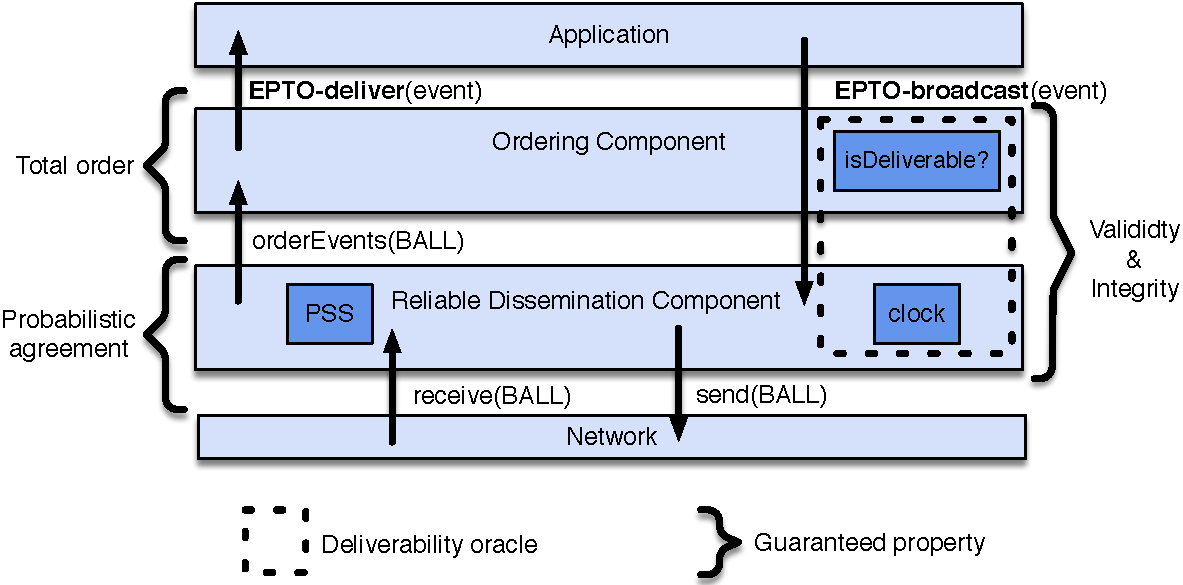
\includegraphics[width=\linewidth]{figures/architecture.pdf}
	\caption{\epto architecture \autocite{matos2015epto}.}
	\label{fig:epto-architecture}
\end{figure}
EpTOTester is a practical implementation of \epto designed to assess the claims made in \autocite{matos2015epto}. Although the implementation was written with benchmarking in mind, the code could be adapted to be used in a real application with only minimal changes to the sources.
\subsection{Architecture}
Figure \ref{fig:epto-architecture} illustrates the architecture of a single replica. An application extending our Application class can broadcast and delivers events. Events broadcasted to the Dissemination component are sent over the network every $\delta$ period. Every events received from the network are analyzed by the Dissemination component to find out whether they need to be propagated further or not according to their Time To Live (TTL).They are then sent to the ordering component so that \epto can determine whether to deliver these events or not and in which order. The order is based on the timestamp of the events given by the logical clock and their broadcaster ID in case of a tie. The network layer communication is done using UDP and a PSS CYCLON to gather a random view of peers. To obtain an initial random view, we contact an independent tracker that keeps track of dead and alive nodes in the system. We want to emphasize that the tracker is not obligatory. In practice it works well, but using DHTs is certainly a possibility.
\subsection{Implementation}
We implemented the data sent as randomly generated UUIDs. We implemented our own PSS CYCLON operating on its own port. When implementing \jgroups we had to use TCPGOSSIP instead of the traditional MULTICAST option to coordinate peers. This is not a problem as in a real WAN \jgroups could not rely on MULTICAST. The framework is open-sourced on Github.
\subsection{Deployment}
To deploy \epto effectively we effectively need two different services. One containing the tracker and one containing all \epto replicas. This is achieved using Docker and especially the new Docker Swarm introduced in Docker 1.12. This lets us have a unified way of deploying our benchmarks locally or remotely on vastly different clusters with minimal tweaks. Every benchmark is launched through a Python script available on the master mode. This script handles everything, from starting benchmarks, scaling the cluster during a churn and collecting results. All \epto parameters are customizable by using options provided through this script.
Gradle is used to automate the image building in the python scripts. Finally, a script is provided to push the images to a repository accessible to the remote cluster and to push the benchmarking script on the master node. \jgroups deployment is much the same. \jt{I should create a figure showcasing the complete architecture}
\subsection{Fault Injection}
Our framework supports the ability to inject synthetic and real traces thanks to the work done in \autocite{vaucher2016erasure}, although the synthetic churn was improved to support adding and removing nodes at the same time.